\documentclass{acm_proc_article-sp}

\begin{document}

\title{Project-060: I523: Project:\\ Dynamics of International Migration}

\numberofauthors{1} 
\author{
\alignauthor
FG-16-DG-4074: Yee Sern Tan\\
       \affaddr{Indiana University Bloomington\\
       IN 47408, USA}\\
       \email{yeestan@indiana.edu}
       }

\date{20 April 2013}


\maketitle
\begin{abstract}
The dynamics of bilateral migration is analyzed on a global scale with data from years 2000 and 2010. Indicators such as GDP per capita and Gini coefficient are considered as predictors of migration data. There is observed significant positive correlation between immigration and log GDP per capita. The largest trends and communities in global migration are stated briefly.
\end{abstract}

\section{Introduction}
International migration is an evolving topic. Most analyses have anchored on qualitative measures, with different countries presenting a varied number of perspectives on how the topic is to be approached. The instabilities in politics and society and the differences in economic opportunities have been the major contributors to migration. The measures applied being subject to provision by each individual country, and assuming that they provide an accurate estimate, an endeavor into understanding the quantitative patterns underlying these trends is desired and is here studied at the global scale.

\section{Data}
The sources of data are OECD, UN and World Bank websites \cite{drc, oecd}. The data from World Bank website cannot be automatically downloaded, as it was sourced from \cite{worldbank_migr, worldbank_other} after an interactive selection of fields that apply to the file to be downloaded. The available files can be found in the data folder.

\section{Analysis}
It is well known that economic factors are driving factors of migration. An analysis proceeds by considering the effect of GDP, Gini coefficient, and distances between centers of population.

\subsection{Wealth}
The logarithmic scale of GDP per capita, a natural comparative measure of wealth, is used here. With year 2000 migration data from \cite{drc}, and economic and population data from \cite{worldbank_other}, regression \cite{scikit-learn} is done for migration rate (response variable) from one country to another country versus relative log GDP per capita (covariate), weighted with the product of populations of both countries. The output is shown in Figure \ref{fig:reg2000}. (This rate can exceed 1, explained by the emigration rate of the emigrating country to the immigrating country, divided by the immigrating country's share of world population. For an illustration, if 1\% of the population of country A migrates to country B, while country B has 0.1\% of world population, the rate is 10. With this measure, by far, the maximal migrating rate is observed from Dominica to Antigua \& Barbuda. Their respective populations are 69679 and 77648, with a total number of migrants 2667.) Since there are small numbers in small countries exhibiting exorbitant rates of migration, the plot with regression line is zoomed-in to gain a clearer view of the larger trend. 

\begin{figure}[h]
    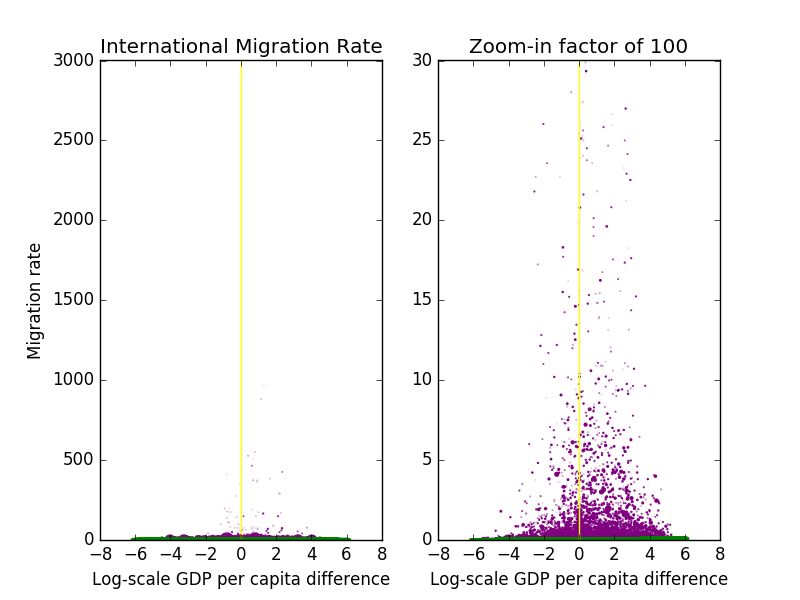
\includegraphics[width=\columnwidth, keepaspectratio=true]{GDP_regression_2000.png}
    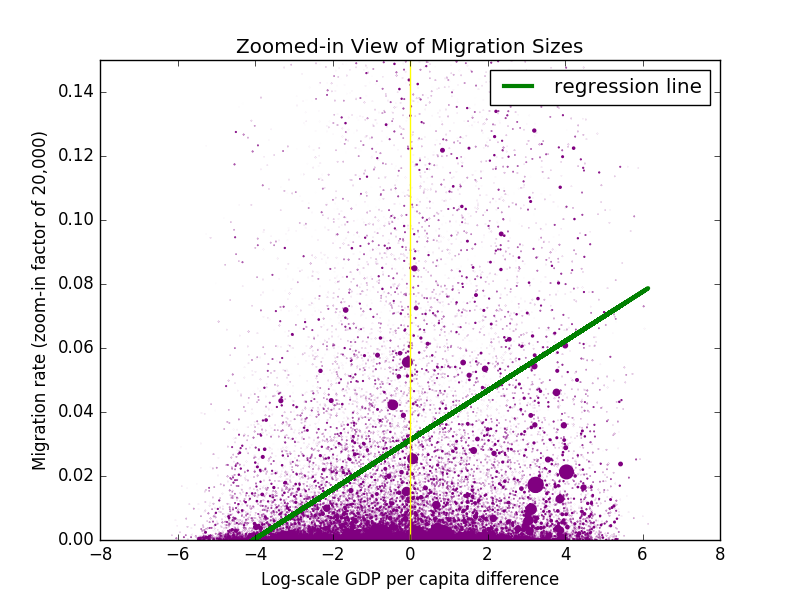
\includegraphics[width=\columnwidth, keepaspectratio=true]{GDP_regression_zoom_2000.png}
    \caption{2000 Migration Rates over Differences in Wealth}
    \label{fig:reg2000}
\end{figure}

There is observed positive correlation signifying emigration from poorer countries to richer countries. In the plots, the points to the right of the yellow vertical line are migrations from poorer to richer countries. Within the plots, there is a cut-off for scale, where points that are too small are not displayed, which is why many migration data from richer to poorer countries do not qualify in the plot. Also, most of the points are far from the regression line, displaying that GDP alone is insufficient to predict migration. The distribution of migrant numbers over differences in economic level is plotted out after smoothing with a Gaussian kernel (Figure \ref{fig:kern2000}). 

\begin{figure}[h]
    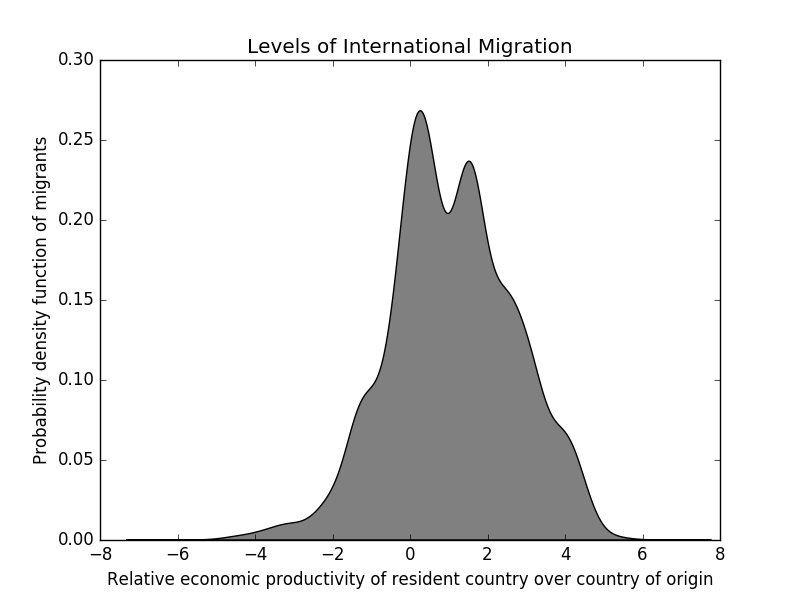
\includegraphics[width=\columnwidth, keepaspectratio=true]{Smoothed_Density_Estimator2000.png}
    \caption{Year 2000 Smoothed Density Estimator of Total Migrants Over Differences in Wealth}
    \label{fig:kern2000}
\end{figure}

The migration rate (divided over total population) for larger countries tend to be smaller, since getting out of a large country often means traveling long distances, which lowers migration especially when transportation is not readily available. Consequentially there should be higher rates of intranational migration, which faces a severe shortage of records and data on number of migrants to be analyzed even on a regional scale.

Analysis of time-series on migration has not been done, mainly due to missingness in data and inconsistent definitions. Although the data on year 2010 \cite{oecd} has a fine breakdown into categories such as gender and age, it has only 40 countries of immigrating countries and is severely impaired in its analysis by the missingness of data. With some forethought, analysis by gender and age at global scales would not provide much information, for they correspond to social issues that are best dealt locally. Furthermore, the country code provided in the data is not consistent. For example, some use EURO while others divide into individual countries; some data have USSR and non-updated national borders as country of birth. Our analysis assumes that the country of birth to be the citizenship country (or the emigrating country), which may not be the case, further reflecting the difficulty that arises due to inhomogeneous data. Similar to the data on 2000, the 2010 data are processed to regress with GDP levels then, and its density is smoothed out with Gaussian kernel and plotted (Figures \ref{fig:reg2010} and \ref{fig:kern2010}).

\begin{figure}[ht]
    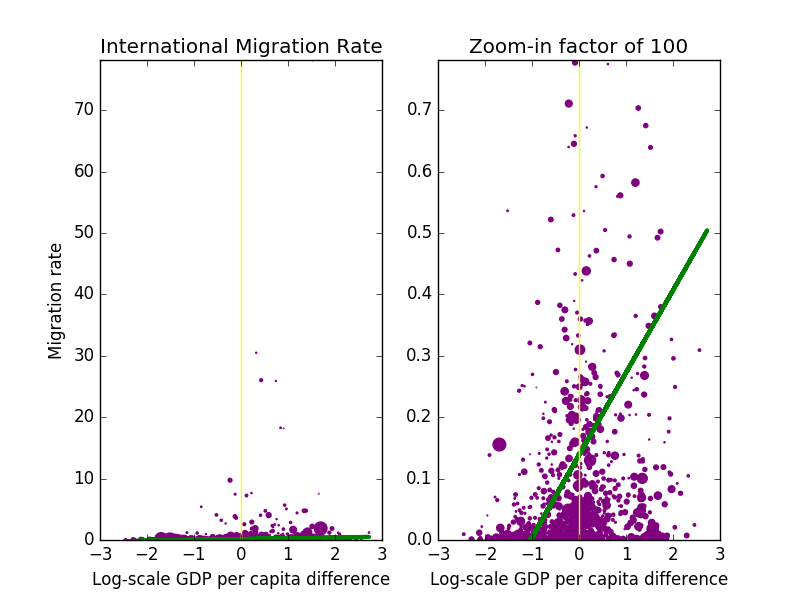
\includegraphics[width=\columnwidth, keepaspectratio=true]{GDP_regression_2010.png}
    \caption{2010 Migration Rates over Differences in Wealth}
    \label{fig:reg2010}
\end{figure}

\begin{figure}[ht]
    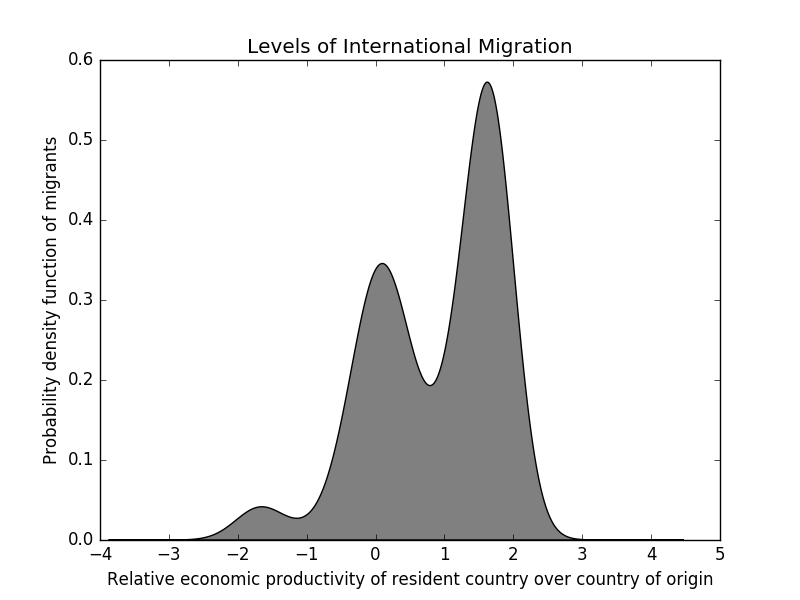
\includegraphics[width=\columnwidth, keepaspectratio=true]{Smoothed_Density_Estimator2010.png}
    \caption{Year 2010 Smoothed Density Estimator of Total Migrants Over Differences in Wealth}
    \label{fig:kern2010}
\end{figure}

\subsection{Equality}
The number of countries that have Gini coefficient data provided for year 2000 is very limited (only 41), and therefore, it is very much subject to selection bias. There is also a lack of clear evaluation of the Gini coefficient, as a one-dimensional variable between 0 and 1, that aims to describe distribution of wealth over a broad spectrum of society. We regress for $a_1x_1 + a_2x_2 = y$, where the response $y$ is a vector of migration between pairs of countries, $x_1$ is the corresponding difference in log GDP, and $x_2$ the difference in Gini coefficient. The linear scale is resized by substituting $x_1$ with $x_1 (\max_i x_{2i} - \min_i x_{2i})/(\max_i x_{1i} - \min_i x_{1i}) $ such that extremal values of GDP per capita and Gini coefficient fit exactly into a square to get a rough idea. The regression coefficients from the observed data show that the dependency of migration on Gini coefficient by a factor of $a_2$ is weakly negative (more migration to countries with lower coefficients), and this scale-invariant dependency is weak (only $a_2/a_1 = 0.0194$ that of GDP per capita).

\subsection{GDP Prediction Strength}
Having established that GDP per capita is a good predictor of global trends in migration, we now analyze individual countries. The prediction strength of GDP per capita on migration direction of individual countries are considered. Separately for immigration and emigration, the weighted correlation coefficient between migrant number and relative log GDP per capita is calculated for each country. This correlation is positive for 110 (immigration) and 122 (emigration) among 180 countries. Interactive maps can be displayed on a browser upon running a script (visualization.sh, see README).

\subsection{Distance}
In this paper, the center of population of a country means the estimated centroid of population. Based on differences in the ability to travel and availability of data, the analysis of effect of the center of population on migration is limited to European countries \cite{hamerly}. After regressing out the confounding effects of GDP by leveling out the contribution of GDP to migration, we obtain the expected distribution of migrants with respect to distance. Further, the values in this distribution is divided by the actual distribution of populations for each distance, to neutralize the effect of base-rate of distance. It is found, that the distribution of this ratio, the tendency of migration, is closest explained with approximately inversely proportional to the 1.4397-th power of distance (Haversine distance between centers of population). $r \approx d^{-1.439}$. The method for fitting the power-law exponent 
$\alpha = 1 + n [\sum_{i=1}^n \ln \frac{x_{1i}}{\min_j{x_1j} - 0.5} ]^{-1}$ 
can be found in \cite{clauset, newman05}. A sketch of complementary cumulative distribution is compared with pure power-law distribution (straight line) in Figure \ref{fig:ccdf}. 

\begin{figure}[H]
    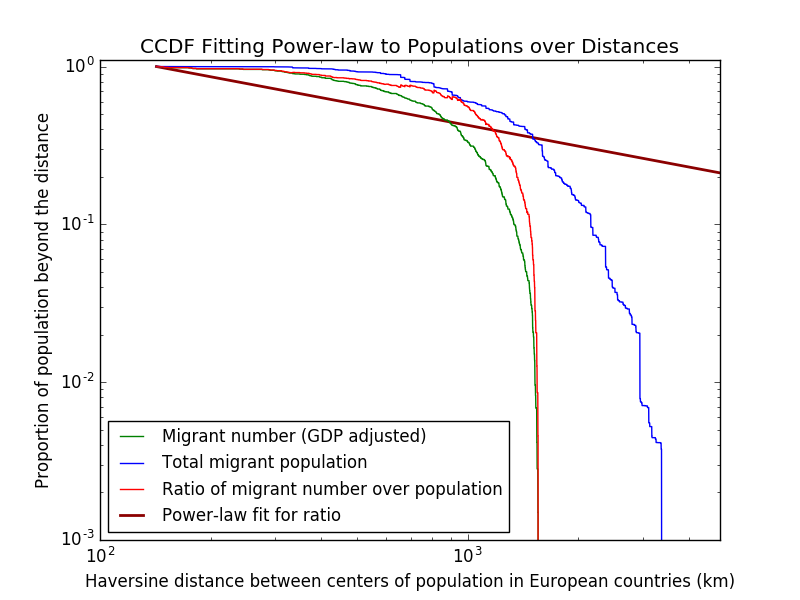
\includegraphics[width=\columnwidth, keepaspectratio=true]{ccdf_distance.png}
    \caption{CCDF of Tendency for Migration within Europe, 2000}
    \label{fig:ccdf}
\end{figure}

From the plot (green curve) approximately half of migrants within the continent live in country that is within 900 km of citizenship country. The power-law fit is far from conclusive, but it does suggest that the power exponent increases with distance. The formulation for Europe gets a good picture of the model much because it is generally densely populated and closely connected with a large number of countries. Northern Europe, which is sparsely populated, can be remedied as its centers of populations are more focused toward the south. Russia, however, would not fit into the model with its center of population, because its migrants within Europe tend to be much closer to these neighbors than its center of population, which considers even to the population of the Far East. Therefore, it is removed for the purpose of this analysis.

\subsection{Largest Data}

Among pair of countries, the top data both for total bidirectional migration, and by far the top for net migration, are from Mexico to United States \cite{mpi}. This large statistic has been building up over the years until the late 2000's and has been a contributor of social issues. Coming in second over total migration is between the Russian Federation and Ukraine. Contrasting with the previous example where migration is predominantly unidirectional, this example shows high migration data in both directions. Given the relative small size of Ukraine, this situation reflects itself the Ukrainian crisis in 2013  \cite{osw}. (See Tables \ref{tab:net} and \ref{tab:total}.)

\begin{table}[h]
\centering
\caption{Top 5 Country Pairs for Net Migration (2000)}
\begin{tabular}{|l|l|l|}
\cline{1-3}
Immigration   & Emigration & Net flow   \\ \cline{1-3}
United States & Mexico     & 8,994,582  \\ \cline{1-3}
India         & Bangladesh & 2,847,672  \\ \cline{1-3}
Hong Kong     & China      & 2,192,983  \\ \cline{1-3}
Pakistan      & Bangladesh & 1,487,952  \\ \cline{1-3}
France        & Algeria    & 1,330,392  \\ \cline{1-3}
\end{tabular}
\label{tab:net}
\end{table}

\begin{table}[h]
\centering
\caption{Top 5 Country Pairs for Total Migrants (2000)}
\begin{tabular}{|l|l|l|}
\cline{1-3}
Country 1     & Country 2  & Total Migrants \\ \cline{1-3}
United States & Mexico     & 9,678,856      \\ \cline{1-3}
Russia        & Ukraine    & 8,428,173      \\ \cline{1-3}
Russia        & Kazakhstan & 4,774,397      \\ \cline{1-3}
India         & Bangladesh & 4,764,016      \\ \cline{1-3}
China         & Hong Kong  & 2,193,867      \\ \cline{1-3}
\end{tabular}
\label{tab:total}
\end{table}

The data applied was in year 2000, a decade before the Arab spring uprising that caused instabilities across the Middle East resulting in mass migration to European countries --- the largest in scale since the second World War ended. This wave of migration presents an issue of controversy mixed with humanitarian crisis. After the neighboring countries in the Middle East, Europe has been taking up the largest number, with the largest group of asylum seekers and refugees estimated to be in Germany, numbering to about 1 million \cite{million}. While many of these refugees would return to their homeland if and when the situation is to improve, their presence brings us into consideration over how immigration rules are to be enforced, and asylum seekers are to be treated, as well as the need or ability to accommodate large numbers of people in the face of crisis. With the presence of numbers that evade detection as they trespass border, and with the dynamically changing nature of such statistics, an analysis will prove challenging and is not done here.

\subsection{Communities of Migration}
The project proposal mentioned about generating "clusters" of countries with high migration between each other. Now that the migration relation is a bilateral relation between the emigrating country and immigrating country, it is conceptually more sensible to represent this relation as a graph. Instead of computing clusters in a vector space of dimension the number of countries, we compute "communities" within the graph. Here, the idea of communities are the groups of countries where migration within the group is larger than migration crossing the borders of the groups.
\\
We construct a metric to signify weights of the edges of the graph. To simplify analysis, this graph is assumed to be undirected, that is, we only quantify the total (bidirectional) number of migrants between two countries and put aside the direction of migration. The weight is computed proportional to 
$\frac{m_{ij}+m_{ji}}{m_{i,all}+m_{all,i}+m_{j,all}+m_{all,j}}, $
where $m_{ij}$ is the number of migrants of country $i$ in country $j$,  $m_{i,all}$ is the total number of emigrants of country $i$,
and $m_{all,i}$ is the total number of immigrants in country $i$. This is a metric that yields a stable result, in favor of placing higher weights on large countries. The weight is multiplied by the total number of countries involved to get values close to 1. A threshold of 0.5 is applied to cut off weak migration relations. 
\\
The Louvain method is then applied for ease of incorporating modularity maximization of large graphs \cite{louvain}. The result obtained has 26 communities. Using modularity has the setback of not being able to detect communities below a certain resolution limit. Only the 12 communities above the resolution limit are considered (see Figure \ref{fig:comm} and supplementary material). This generation of communities may spark worries about the possibility of a world that is fragmented into various groups that have little interaction with each other. To measure the extent of fragmentation, the modularity score \cite{newman06}, a scale of -1 to 1 indicating how likely migration is to occur within communities, versus with randomly selected, is computed as 0.6885 for reference. The communities are:
\begin{itemize}
\item Much of Europe, North Africa, Turkey and Northern corner of South America. 
\item East Asia, North America, UK \& Ireland, Australia \& New Zealand and Southeast Asia.
\item Central, East and South Africa. 
\item Middle East and South Asia.
\item Western Africa.
\item Central Asia and Eastern Europe.
\item Northern Europe and East Africa.
\item The Caribbean.
\item South America. 
\item Archipelagic Oceania.
\item Central Europe.
\item Central America.
\end{itemize}

\begin{figure}[h]
    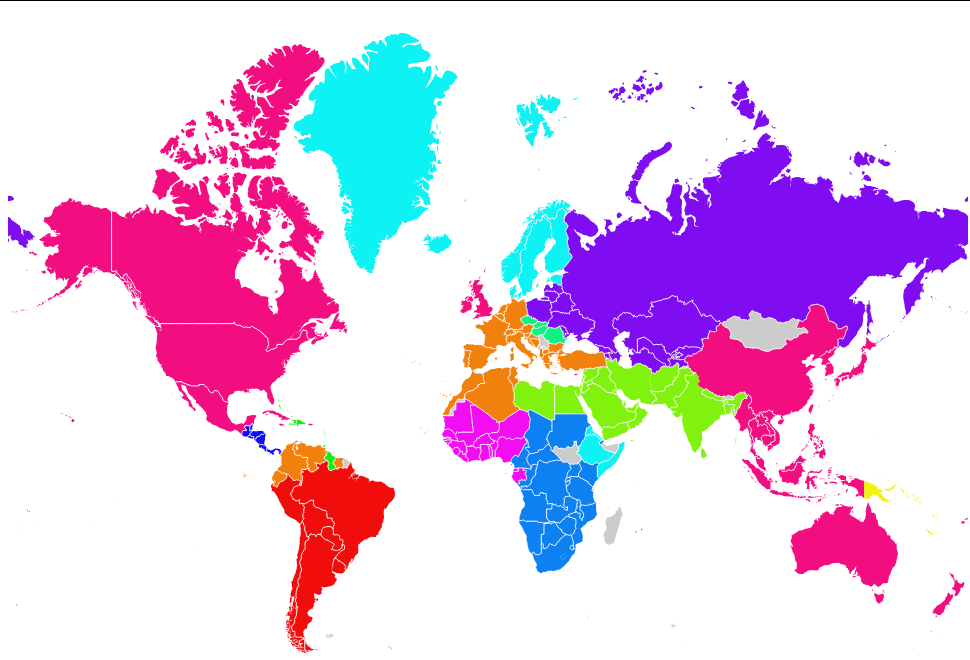
\includegraphics[width=\columnwidth, keepaspectratio=true]{Migration_communities.png}
    \caption{Communities of World Migration (2000)}
    \label{fig:comm}
\end{figure}

\section{Visualization}
Javascript code was obtained from VIDA \cite{vida}. Modifications were made from it to generate world maps that have countries colored according to immigrating, emigration and migrant community statistics. The code requires an account with the website to retrieve, and therefore, it is not set to auto-download.

\section{Conclusions}
This analysis project touches on the global effects of wealth, inequality, and distance on migration statistics. The effectiveness of these statistics are also considered. Loose communities are also generated.
\\
All the results of this analysis project are simply functions of the obtained data, marking major trends, without touching more complex issues such as quality of life, treatment of foreigners, duration of migration and the social issues underlying these factors. A comprehensive review of global migration will require collaboration between governments, providing data that are up to standard as well as homogeneous. Except when there is need for public information, there appears to be not much motivation to set up a complete global and centralized source of public repository regarding migrants, compared with other more prominent national interests. The most complete data sourced, on a global scale, dates to 2000. The outlook for reliable collation of data is at-best uncertain in the near future.

\section{Acknowledgments}
The availability of migration data by OECD, World Bank and United Nations, and that of open source programs: the python programming language and many of its packages enabled this project. The author is thankful for the online sources available, on areas including: getting contents from spreadsheets \cite{xlrd}, loading html file from python \cite{html}, and selecting colors for communities within the world map \cite{color}.

\bibliographystyle{IEEEtran}
\bibliography{references}

\balancecolumns 

\end{document}
